%%%%%%%%%%%%%%%%%%%%%%%%%%%%%%%%%%%%%%%%%
% Programming/Coding Assignment
% LaTeX Template
%
% This template has been downloaded from:
% http://www.latextemplates.com
%
% Original author:
% Ted Pavlic (http://www.tedpavlic.com)
%
% Note:
% The \lipsum[#] commands throughout this template generate dummy text
% to fill the template out. These commands should all be removed when 
% writing assignment content.
%
% This template uses a Perl script as an example snippet of code, most other
% languages are also usable. Configure them in the "CODE INCLUSION 
% CONFIGURATION" section.
%
%%%%%%%%%%%%%%%%%%%%%%%%%%%%%%%%%%%%%%%%%

%----------------------------------------------------------------------------------------
%	PACKAGES AND OTHER DOCUMENT CONFIGURATIONS
%----------------------------------------------------------------------------------------

\documentclass{article}

\usepackage{fancyhdr} % Required for custom headers
\usepackage{lastpage} % Required to determine the last page for the footer
\usepackage{extramarks} % Required for headers and footers
\usepackage[usenames,dvipsnames]{color} % Required for custom colors
\usepackage{graphicx} % Required to insert images
\usepackage{subcaption}
\usepackage{listings} % Required for insertion of code
\usepackage{courier} % Required for the courier font
\usepackage{lipsum} % Used for inserting dummy 'Lorem ipsum' text into the template

% % % % % % % % %
\usepackage{listings}
\usepackage{color}

\definecolor{dkgreen}{rgb}{0,0.6,0}
\definecolor{gray}{rgb}{0.5,0.5,0.5}
\definecolor{mauve}{rgb}{0.58,0,0.82}

\lstset{frame=tb,
  language=Python,
  aboveskip=3mm,
  belowskip=3mm,
  showstringspaces=false,
  columns=flexible,
  basicstyle={\small\ttfamily},
  numbers=none,
  numberstyle=\tiny\color{gray},
  keywordstyle=\color{blue},
  commentstyle=\color{dkgreen},
  stringstyle=\color{mauve},
  breaklines=true,
  breakatwhitespace=true,
  tabsize=3
}
% % % % % % % % %
% Margins
\topmargin=-0.45in
\evensidemargin=0in
\oddsidemargin=0in
\textwidth=6.5in
\textheight=9.0in
\headsep=0.25in

\linespread{1.1} % Line spacing

% Set up the header and footer
\pagestyle{fancy}
\lhead{\hmwkAuthorName} % Top left header
\chead{\hmwkClass\ (\hmwkClassTime): \hmwkTitle} % Top center head
\rhead{\firstxmark} % Top right header
\lfoot{\lastxmark} % Bottom left footer
\cfoot{} % Bottom center footer
\rfoot{Page\ \thepage\ of\ \protect\pageref{LastPage}} % Bottom right footer
\renewcommand\headrulewidth{0.4pt} % Size of the header rule
\renewcommand\footrulewidth{0.4pt} % Size of the footer rule

\setlength\parindent{0pt} % Removes all indentation from paragraphs

%----------------------------------------------------------------------------------------
%	CODE INCLUSION CONFIGURATION
%----------------------------------------------------------------------------------------

\definecolor{MyDarkGreen}{rgb}{0.0,0.4,0.0} % This is the color used for comments
\lstloadlanguages{Perl} % Load Perl syntax for listings, for a list of other languages supported see: ftp://ftp.tex.ac.uk/tex-archive/macros/latex/contrib/listings/listings.pdf
\lstset{language=Perl, % Use Perl in this example
        frame=single, % Single frame around code
        basicstyle=\small\ttfamily, % Use small true type font
        keywordstyle=[1]\color{Blue}\bf, % Perl functions bold and blue
        keywordstyle=[2]\color{Purple}, % Perl function arguments purple
        keywordstyle=[3]\color{Blue}\underbar, % Custom functions underlined and blue
        identifierstyle=, % Nothing special about identifiers                                         
        commentstyle=\usefont{T1}{pcr}{m}{sl}\color{MyDarkGreen}\small, % Comments small dark green courier font
        stringstyle=\color{Purple}, % Strings are purple
        showstringspaces=false, % Don't put marks in string spaces
        tabsize=5, % 5 spaces per tab
        %
        % Put standard Perl functions not included in the default language here
        morekeywords={rand},
        %
        % Put Perl function parameters here
        morekeywords=[2]{on, off, interp},
        %
        % Put user defined functions here
        morekeywords=[3]{test},
       	%
        morecomment=[l][\color{Blue}]{...}, % Line continuation (...) like blue comment
        numbers=left, % Line numbers on left
        firstnumber=1, % Line numbers start with line 1
        numberstyle=\tiny\color{Blue}, % Line numbers are blue and small
        stepnumber=5 % Line numbers go in steps of 5
}

% Creates a new command to include a perl script, the first parameter is the filename of the script (without .pl), the second parameter is the caption
\newcommand{\perlscript}[2]{
\begin{itemize}
\item[]\lstinputlisting[caption=#2,label=#1]{#1.pl}
\end{itemize}
}

%----------------------------------------------------------------------------------------
%	DOCUMENT STRUCTURE COMMANDS
%	Skip this unless you know what you're doing
%----------------------------------------------------------------------------------------

% Header and footer for when a page split occurs within a problem environment
\newcommand{\enterProblemHeader}[1]{
\nobreak\extramarks{#1}{#1 continued on next page\ldots}\nobreak
\nobreak\extramarks{#1 (continued)}{#1 continued on next page\ldots}\nobreak
}

% Header and footer for when a page split occurs between problem environments
\newcommand{\exitProblemHeader}[1]{
\nobreak\extramarks{#1 (continued)}{#1 continued on next page\ldots}\nobreak
\nobreak\extramarks{#1}{}\nobreak
}

\setcounter{secnumdepth}{0} % Removes default section numbers
\newcounter{homeworkProblemCounter} % Creates a counter to keep track of the number of problems

\newcommand{\homeworkProblemName}{}
\newenvironment{homeworkProblem}[1][Part \arabic{homeworkProblemCounter}]{ % Makes a new environment called homeworkProblem which takes 1 argument (custom name) but the default is "Problem #"
\stepcounter{homeworkProblemCounter} % Increase counter for number of problems
\renewcommand{\homeworkProblemName}{#1} % Assign \homeworkProblemName the name of the problem
\section{\homeworkProblemName} % Make a section in the document with the custom problem count
\enterProblemHeader{\homeworkProblemName} % Header and footer within the environment
}{
\exitProblemHeader{\homeworkProblemName} % Header and footer after the environment
}

\newcommand{\problemAnswer}[1]{ % Defines the problem answer command with the content as the only argument
\noindent\framebox[\columnwidth][c]{\begin{minipage}{0.98\columnwidth}#1\end{minipage}} % Makes the box around the problem answer and puts the content inside
}

\newcommand{\homeworkSectionName}{}
\newenvironment{homeworkSection}[1]{ % New environment for sections within homework problems, takes 1 argument - the name of the section
\renewcommand{\homeworkSectionName}{#1} % Assign \homeworkSectionName to the name of the section from the environment argument
\subsection{\homeworkSectionName} % Make a subsection with the custom name of the subsection
\enterProblemHeader{\homeworkProblemName\ [\homeworkSectionName]} % Header and footer within the environment
}{
\enterProblemHeader{\homeworkProblemName} % Header and footer after the environment
}

%----------------------------------------------------------------------------------------
%	NAME AND CLASS SECTION
%----------------------------------------------------------------------------------------

\newcommand{\hmwkTitle}{Project 3} % Assignment title
\newcommand{\hmwkDueDate}{Face Recognition and Classification with Eigenfaces} % Due date
\newcommand{\hmwkClass}{CSC320} % Course/class
\newcommand{\hmwkClassTime}{L0101} % Class/lecture time
\newcommand{\hmwkAuthorName}{Ramaneek Gill and Ryan D'Souza} % Your name

%----------------------------------------------------------------------------------------
%	TITLE PAGE
%----------------------------------------------------------------------------------------

\title{
\vspace{2in}
\textmd{\textbf{\hmwkClass:\ \hmwkTitle}}\\
\normalsize\vspace{0.1in}\small{\hmwkDueDate}\\
\vspace{0.1in}
\vspace{3in}
}

\author{\textbf{\hmwkAuthorName}}
%\date{} % Insert date here if you want it to appear below your name

%----------------------------------------------------------------------------------------

\begin{document}

\maketitle
\clearpage




%----------------------------------------------------------------------------------------
%	PART 1
%----------------------------------------------------------------------------------------

\begin{homeworkProblem}

\noindent

The dataset of faces used were of popular celebrities (mainly 'Aaron Eckhart', 'Adam Sandler', 'Adrien Brody', 'Andrea Anders', 'Ashley Benson', 'Christina Applegate', 'Dianna Agron', and 'Gillian Anderson'). The images are or size 32 by 32 and have been grayscaled by using 0.299 intensity from the red channel, 0.587 from the green channel and 0.114 from the blue channel, just like in project 2. As shown in Figure 1 the cropped out faces are fairly accurate, most images can be aligned with each other but some images only show the side of the face. Thanks to a fairly large dataset we shouldn't be concerned about these 'outliers'.

\begin{figure}[h!]
        \centering
        \begin{subfigure}[b]{0.33\textwidth}
                \includegraphics[width=\textwidth]{cropped/agron3.jpg}
                \caption{An example of a less than desirable image for facial recognition}
                \label{fig:1a}
        \end{subfigure}%
        ~
        \begin{subfigure}[b]{0.33\textwidth}
                \includegraphics[width=\textwidth]{cropped/anderson16.jpg}
                \caption{A good image for face detection}
                \label{fig:1b}
        \end{subfigure}
        \begin{subfigure}[b]{0.33\textwidth}
                \includegraphics[width=\textwidth]{cropped/eckhart8.jpg}
                \caption{An alright image for face detection}
                \label{fig:1c}
        \end{subfigure}
        \caption{A subset of the dataset of images used}\label{fig:dataset}
\end{figure}

\end{homeworkProblem}

%----------------------------------------------------------------------------------------
%	PART 2
%----------------------------------------------------------------------------------------
\begin{homeworkProblem}

\noindent

The dataset was seperated into 100 training images, 10 validation images, and 10 test images. This was done by just filling an array until it was full, the code is provided in the \texttt{getData()} function in the source code (for your convenience it is located in the last section of the report). Figure 2 shows 25 eigenfaces (of the 800 possible ones, 100 for each actor for a total of 8 actors) and the mean face of the training set.

\begin{figure}[h!]
        \centering
        \begin{subfigure}[b]{0.75\textwidth}
                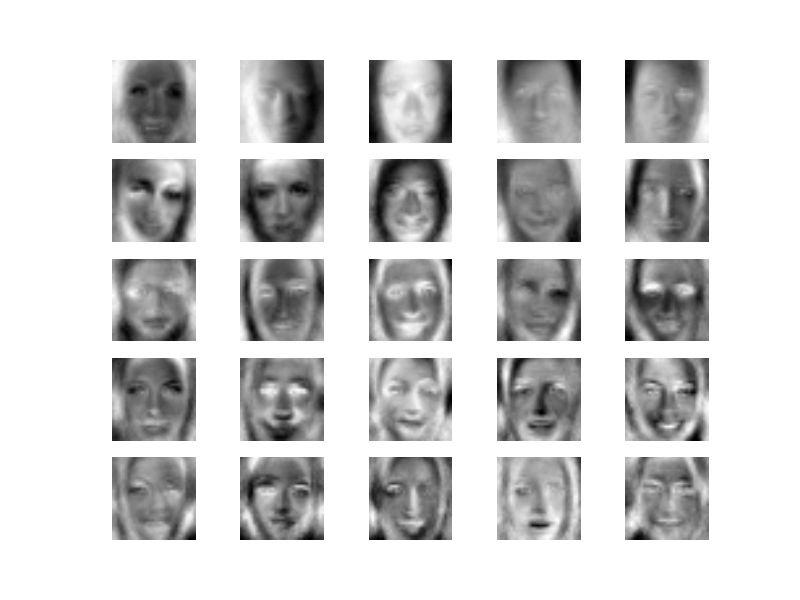
\includegraphics[width=\textwidth]{report/display_save_25_comps.jpg}
                \caption{25 eigenfaces from the 800 in our dataset}
                \label{fig:2a}
        \end{subfigure}%
        ~
        \begin{subfigure}[b]{0.3\textwidth}
                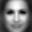
\includegraphics[width=\textwidth]{report/mean_face.jpg}
                \caption{The mean face of the eigenspace of 800 eigenfaces}
                \label{fig:2b}
        \end{subfigure}
        \caption{Data generated from part 2}\label{fig:2}
\end{figure}

\end{homeworkProblem}

%----------------------------------------------------------------------------------------
%	PART 3
%----------------------------------------------------------------------------------------
\begin{homeworkProblem}

\noindent

The results from running \texttt{p3.py}:
\\
Training, validation, and test sets created!\\
Projection matrix and mean eigenface computed!\\
This match was incorrect, validation image 0 incorrectly matched actor 0 with  4\\
This match was incorrect, validation image 1 incorrectly matched actor 0 with  2\\
This match was incorrect, validation image 3 incorrectly matched actor 0 with  2\\
This match was incorrect, validation image 4 incorrectly matched actor 0 with  2\\
This match was incorrect, validation image 6 incorrectly matched actor 0 with  1\\
Performance on the validation set using 2 eigenfaces was:  22.5\\
Best setting for face recognition is to use 2 eigenfaces\\
Performance on the validation set using 5 eigenfaces was:  38.75\\
Best setting for face recognition is to use 5 eigenfaces\\
Performance on the validation set using 10 eigenfaces was:  47.5\\
Best setting for face recognition is to use 10 eigenfaces\\
Performance on the validation set using 20 eigenfaces was:  61.25\\
Best setting for face recognition is to use 20 eigenfaces\\
Performance on the validation set using 50 eigenfaces was:  66.25\\
Best setting for face recognition is to use 50 eigenfaces\\
Performance on the validation set using 80 eigenfaces was:  65.0\\
Best setting for face recognition is to use 50 eigenfaces\\
Performance on the validation set using 100 eigenfaces was:  66.25\\
Best setting for face recognition is to use 50 eigenfaces\\
Performance on the validation set using 150 eigenfaces was:  66.25\\
Best setting for face recognition is to use 50 eigenfaces\\
Performance on the validation set using 200 eigenfaces was:  67.5\\
Best setting for face recognition is to use 200 eigenfaces\\
Performance on the test set using 200 eigenfaces was:  50.0\\
\\
Figure 3a,4a,5a,6a,7a show the 0th, 1st, 3rd, 4th, and 6th validation images in the validation set were incorrectly recognized as the images from the training set as shown in Figure 3b,4b,5b,6b,7b respectively when using only 2 eigenfaces to compute facial recognitions.

\begin{figure}[h!]
        \centering
        \begin{subfigure}[b]{0.2\textwidth}
                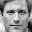
\includegraphics[width=\textwidth]{report/1 Aaron Eckhart incorrectly matched.jpg}
                \caption{This image was incorrectly matched with Figure 3b}
                \label{fig:3a}
        \end{subfigure}%
        ~
        \begin{subfigure}[b]{0.2\textwidth}
                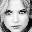
\includegraphics[width=\textwidth]{report/1 Ashley Benson with.jpg}
                \caption{This recognition was computed using only 2 eigenfaces}
                \label{fig:3b}
        \end{subfigure}
        \caption{Data generated from part 3}\label{fig:3}
\end{figure}

%2

\begin{figure}[h!]
        \centering
        \begin{subfigure}[b]{0.2\textwidth}
                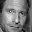
\includegraphics[width=\textwidth]{report/2 Aaron Eckhart incorrectly matched.jpg}
                \caption{This image was incorrectly matched with Figure 4b}
                \label{fig:4a}
        \end{subfigure}%
        ~
        \begin{subfigure}[b]{0.2\textwidth}
                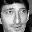
\includegraphics[width=\textwidth]{report/2 Adrien Brody with.jpg}
                \caption{This recognition was computed using only 2 eigenfaces}
                \label{fig:4b}
        \end{subfigure}
        \caption{Data generated from part 3}\label{fig:4}
\end{figure}

%3

\begin{figure}[h!]
        \centering
        \begin{subfigure}[b]{0.2\textwidth}
                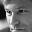
\includegraphics[width=\textwidth]{report/3 Aaron Eckhart incorrectly matched.jpg}
                \caption{This image was incorrectly matched with Figure 5b}
                \label{fig:5a}
        \end{subfigure}%
        ~
        \begin{subfigure}[b]{0.2\textwidth}
                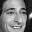
\includegraphics[width=\textwidth]{report/3 Adrien Brody with.jpg}
                \caption{This recognition was computed using only 2 eigenfaces}
                \label{fig:5b}
        \end{subfigure}
        \caption{Data generated from part 3}\label{fig:5}
\end{figure}

%4

\begin{figure}[h!]
        \centering
        \begin{subfigure}[b]{0.2\textwidth}
                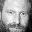
\includegraphics[width=\textwidth]{report/4 Aaron Eckhart incorrectly matched.jpg}
                \caption{This image was incorrectly matched with Figure 6b}
                \label{fig:6a}
        \end{subfigure}%
        ~
        \begin{subfigure}[b]{0.2\textwidth}
                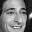
\includegraphics[width=\textwidth]{report/4 Adrien Brody with.jpg}
                \caption{This recognition was computed using only 2 eigenfaces}
                \label{fig:6b}
        \end{subfigure}
        \caption{Data generated from part 3}\label{fig:6}
\end{figure}

%5

\begin{figure}[h!]
        \centering
        \begin{subfigure}[b]{0.2\textwidth}
                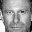
\includegraphics[width=\textwidth]{report/5 Aaron Eckhart incorrectly matched.jpg}
                \caption{This image was incorrectly matched with Figure 7b}
                \label{fig:7a}
        \end{subfigure}%
        ~
        \begin{subfigure}[b]{0.2\textwidth}
                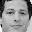
\includegraphics[width=\textwidth]{report/5 Adam Sandler with.jpg}
                \caption{This recognition was computed using only 2 eigenfaces}
                \label{fig:7b}
        \end{subfigure}
        \caption{Data generated from part 3}\label{fig:7}
\end{figure}


\end{homeworkProblem}
\clearpage
%----------------------------------------------------------------------------------------
%	PART 4
%----------------------------------------------------------------------------------------

\begin{homeworkProblem}

\noindent

The output of the program: \\
Performance on the validation set using 2 eigenfaces was:  75.0\\
Performance on the validation set using 5 eigenfaces was:  73.75\\
Performance on the validation set using 10 eigenfaces was:  85.0\\
Performance on the validation set using 20 eigenfaces was:  88.75\\
Performance on the validation set using 50 eigenfaces was:  92.5\\
Performance on the validation set using 80 eigenfaces was:  91.25\\
Performance on the validation set using 100 eigenfaces was:  92.5\\
Performance on the test set using 150 eigenfaces was:  62.5\\
\end{homeworkProblem}

\clearpage

\section{p3.py:}
\begin{lstlisting}



from pylab import *
import numpy as np
import random
import matplotlib.cbook as cbook
import random
import time
from scipy.misc import imread
from scipy.misc import imsave
from scipy.misc import imresize
import matplotlib.image as mpimg
import matplotlib.pyplot as plt
import os


matplotlib
gray()

os.chdir('C:/Users/Ramaneek/SkyDrive/Documents/Github/CSC320-Winter-2014/project 3/')

#global variables
act = ['Aaron Eckhart',  'Adam Sandler',   'Adrien Brody',  'Andrea Anders',    'Ashley Benson',    'Christina Applegate',    'Dianna Agron',  'Gillian Anderson']
training_set = np.zeros((len(act)*100, 32*32)) - 1  #need to use zeros()!!
validation_set = np.zeros((len(act)*10, 32*32)) - 1 #32*32 since a 32x32 matrix is flattened
test_set = np.zeros((len(act)*10, 32*32)) - 1
    
#fills in the global variable data
def getData():
    count_tr = 0 #training
    count_va = 0 #validation
    count_te = 0 #testing
    k = 135 #every actor has at least 135 pics

    for a in act:
        name = a.split()[1].lower()
        for i in range(k):
            if i == k:
                print "You might want to get more images or lower the training set amount"
                exit()
                
            if os.path.isfile("cropped/"+name+str(i)+".jpg"):
                #print "JPG"
                img = imread("cropped/"+name+str(i)+".jpg")
            elif os.path.isfile("cropped/"+name+str(i)+".png"):
                #print "PNG"
                img = imread("cropped/"+name+str(i)+".png")
            else: #couldn't open this image
                #print "trying next image"
                continue

            #need to convert img to gray scale
            gray_img = 0.299*img[:,:,0] + 0.587*img[:,:,1] + 0.114*img[:,:,2]
            #if training_set[(act.index(a)+1)*100,-1] == -1: #get 100 training images for this actor
            if count_tr < (act.index(a)+1) * 100:
                training_set[count_tr][:] = gray_img.flatten()
                count_tr += 1
            elif count_va < (act.index(a)+1) * 10: #get 10 validation images for this actor
                validation_set[count_va][:] = gray_img.flatten()
                count_va += 1
            elif count_te < (act.index(a)+1) * 10: #get 10 test images for this actor
                test_set[count_te][:] = gray_img.flatten()
                count_te += 1
            else: #got all the pictures needed for this actor, move on to next actor
                break
    print "Training, validation, and test sets created!"
    
def pca(X):
    """    Principal Component Analysis
        input: X, matrix with training data stored as flattened arrays in rows
        return: projection matrix (with important dimensions first), variance and mean.
        From: Jan Erik Solem, Programming Computer Vision with Python
        #http://programmingcomputervision.com/
    """
    
    # get dimensions
    num_data,dim = X.shape
    
    # center data
    mean_X = X.mean(axis=0)
    X = X - mean_X
    
    if dim>num_data:
        # PCA - compact trick used
        M = dot(X,X.T) # covariance matrix
        e,EV = linalg.eigh(M) # eigenvalues and eigenvectors
        tmp = dot(X.T,EV).T # this is the compact trick
        V = tmp[::-1] # reverse since last eigenvectors are the ones we want
        S = sqrt(e)[::-1] # reverse since eigenvalues are in increasing order
        for i in range(V.shape[1]):
            V[:,i] /= S
    else:
        # PCA - SVD used
        U,S,V = linalg.svd(X)
        V = V[:num_data] # only makes sense to return the first num_data
    
    # return the projection matrix, the variance and the mean
    print "Projection matrix and mean eigenface computed!"
    return V,S,mean_X
    
def ssd(x, y):
    return sum((x.flatten().astype(float)-y.flatten().astype(float))**2)    
    
def display_save_25_comps(V, im_shape):
    '''Display 25 components in V'''
    figure()
    for i in range(25):
        plt.subplot(5, 5, i+1)
        plt.axis('off')
        gray()
        imshow(V[i,:].reshape(im_shape))
    savefig('report/display_save_25_comps.jpg')  
    show()        

##########################################################################################################################################

getData() #get the data from the cropped images and fill in some of the global variables

projection_M, variance, mean_img = pca(training_set)  #we actually don't even need the variance in this project
display_save_25_comps(projection_M, (32,32))
average_face = np.reshape(mean_img, (32,32)) #keep this to show later on in the report
imsave("report/mean_face.jpg", average_face)

validation_settings = [2, 5, 10, 20, 50, 80, 100, 150, 200] # the top k eigenfaces

#Validation set
max_performance = 0 #for determining the most correct setting for how many eigenfaces to use
best_setting = 0
num_incorrect = 0 #for displaying incorrect matches for reporting purposes

for setting in validation_settings:
    num_correct = 0
    for i in range(validation_set.shape[0]):
        
        #project the validation image on to the eigenface space
        val_proj_img = np.dot(projection_M[:setting], validation_set[i] - mean_img)
        validation_name_index = int(i/10)
        
        #compute the closest projected training face to identify validation_set[i]
        min = Infinity
        for j in range(training_set.shape[0]):
            train_proj_img = np.dot(projection_M[:setting], training_set[j] - mean_img)
            ssd_value = ssd(val_proj_img, train_proj_img)
            if ssd_value < min:
                #print "found new min:", int(j/100)
                min = ssd_value
                #the index of the actor's name
                training_name_index = int(j/100)
                raw_training_name_index = j
                
        #print ssd_value
        #print validation_name, training_name
        if validation_name_index == training_name_index:
            num_correct += 1
            #print "\t found match"
        elif num_incorrect < 5:
            num_incorrect += 1
            print "This match was incorrect, validation image", i, "incorrectly matched actor", validation_name_index, "with ", training_name_index
            imsave("report/"+str(num_incorrect)+"_"+act[validation_name_index]+"_incorrectly_matched.jpg", np.reshape(validation_set[i], (32,32)))
            imsave("report/"+str(num_incorrect)+"_"+act[training_name_index]+"_with.jpg", np.reshape(training_set[raw_training_name_index], (32,32)))
            

    performance = num_correct * 100.0 / validation_set.shape[0]
    print "Performance on the validation set using", setting, "eigenfaces was: ", performance
    if max_performance < performance:
        max_performance = performance
        best_setting = setting
    print "Best setting for face recognition is to use", best_setting, "eigenfaces"
    
#test set
num_correct = 0
for i in range(test_set.shape[0]):
    test_proj_img = np.dot(projection_M[:best_setting], test_set[i] - mean_img)
    test_name_index = int(i/10)
    
    #compute the closest projected training face to identify validation_set[i]
    min = Infinity
    for j in range(training_set.shape[0]):
        train_proj_img = np.dot(projection_M[:best_setting], training_set[j] - mean_img)
        ssd_value = ssd(test_proj_img, train_proj_img)
        if ssd_value < min:
            min = ssd_value
            #the index of the actor's name
            training_name_index = int(j/100)

    if test_name_index == training_name_index:
        num_correct += 1
        
performance = num_correct * 100.0 / test_set.shape[0] 
print "Performance on the test set using", best_setting, "eigenfaces was: ", performance

# Part 3 is done


## Part 4 begin
print "\n\n\nNOW TESTING GENDER RECOGNITION\n\n\n"

#Validation set
max_performance = 0 #for determining the most correct setting for how many eigenfaces to use
best_setting = 0
num_incorrect = 0 #for displaying incorrect matches for reporting purposes

for setting in validation_settings:
    num_correct = 0
    for i in range(validation_set.shape[0]):
        #project the validation image on to the eigenface space
        val_proj_img = np.dot(projection_M[:setting], validation_set[i] - mean_img)
        validation_name_index = int(i/10)
         
        #compute the closest projected training face to identify validation_set[i]
        min = Infinity
        for j in range(training_set.shape[0]):
            train_proj_img = np.dot(projection_M[:setting], training_set[j] - mean_img)
            ssd_value = ssd(val_proj_img, train_proj_img)
            if ssd_value < min:
                min = ssd_value
                training_name_index = int(j/100)
        
        if validation_name_index >= 3 and training_name_index >= 3: #both female
            num_correct += 1
            #print "found match"
        elif validation_name_index < 3 and training_name_index < 3: #both male
            num_correct += 1
        elif num_incorrect < 5:
            num_incorrect += 1
            #print "This match was incorrect, validation image", i, "incorrectly matched actor", validation_name_index, "with ", training_name_index
            #imsave(str(num_incorrect)+act[validation_name_index]+"gender_incorrectly_matched_with"+act[training_name_index]+".jpg")

        
    performance = num_correct * 100.0 / validation_set.shape[0]
    print "Performance on the validation set using", setting, "eigenfaces was: ", performance
    if max_performance < performance:
        max_performance = performance
        best_setting = setting
        
#test set
num_correct = 0
for i in range(test_set.shape[0]):
    test_proj_img = np.dot(projection_M[:best_setting], test_set[i] - mean_img)
    validation_name_index = int(i/10)
    #compute the closest projected training face to identify validation_set[i]
    min = Infinity
    for j in range(training_set.shape[0]):
        train_proj_img = np.dot(projection_M[:best_setting], training_set[j] - mean_img)
        ssd_value = ssd(test_proj_img, train_proj_img)
        if ssd_value < min:
            min = ssd_value
            training_name = int(j/100)

    if validation_name_index >= 3 and training_name_index >= 3: #both female
        num_correct += 1
        #print "found match"
    elif validation_name_index < 3 and training_name_index < 3: #both male
        num_correct += 1
        
performance = num_correct * 100.0 / test_set.shape[0] 
print "Performance on the test set using", best_setting, "eigenfaces was: ", performance

# End part 4
\end{lstlisting}

\section{get data.py}
\begin{lstlisting}
#for downloading the image data
from pylab import *
import numpy as np
import matplotlib.pyplot as plt
import matplotlib.cbook as cbook
import random
import time
from scipy.misc import imread
from scipy.misc import imresize
import matplotlib.image as mpimg
import os
from scipy.ndimage import filters
import urllib


os.chdir('C:/Users/Ramaneek/SkyDrive/Documents/Github/CSC320-Winter-2014/project 3/')

act = ['Aaron Eckhart',  'Adam Sandler',   'Adrien Brody',  'Andrea Anders',    'Ashley Benson',    'Christina Applegate',    'Dianna Agron',  'Gillian Anderson']





def timeout(func, args=(), kwargs={}, timeout_duration=0.5, default=None):
    '''From:
    http://code.activestate.com/recipes/473878-timeout-function-using-threading/'''
    import threading
    class InterruptableThread(threading.Thread):
        def __init__(self):
            threading.Thread.__init__(self)
            self.result = None

        def run(self):
            try:
                self.result = func(*args, **kwargs)
            except:
                self.result = default

    it = InterruptableThread()
    it.start()
    it.join(timeout_duration)
    if it.isAlive():
        return False
    else:
        return it.result

testfile = urllib.URLopener()            


#Note: you need to create the uncropped folder first in order 
#for this to work

for a in act:
    name = a.split()[1].lower()
    i = 0
    for line in open("faces_subset.txt"):
        if a in line:
            # line.split()[-2] gives the x1,y1,x2,y2 coordinates for specific image in this line
            coordinates = line.split()[-2].split(',')  #an array of x1,y1,x2,y2 coordinates
            
            #filename = actorname + number of pics of this actor + filename
            filename = name+str(i)+'.'+line.split()[4].split('.')[-1]
            #A version without timeout (uncomment in case you need to 
            #unsupress exceptions, which timeout() does)
            #testfile.retrieve(line.split()[4], "uncropped/"+filename)
            #timeout is used to stop downloading images which take too long to download
            timeout(testfile.retrieve, (line.split()[4], "uncropped/"+filename), {}, 30)
            print "saved original file:" + filename
            
            if os.path.isfile("uncropped/"+filename): #if the image has been saved
                #need to open this image and crop it
                #no point converting it to grayscale here since imsave saves it as a 3D array
                
                #check to see if image can be read
                try:
                    image_cropped = imread("uncropped/"+filename)
                    image_cropped = image_cropped[int(coordinates[1]):int(coordinates[3]) , int(coordinates[0]):int(coordinates[2])]
                    #now lets resize image to 32x32
                    image_cropped = imresize(image_cropped, (32,32))
                    imsave("cropped/"+filename, image_cropped)
                    print "saved cropped file: " + filename
                except Exception:
                    print "cant open file: " + filename
                    continue 
    
            else:
                print "CONTINUING!!!!!!!!!!!!!!!!!"
                continue

            
            i += 1
    
    
\end{lstlisting}
\end{document}